\documentclass[a4paper,fleqn,usenatbib]{mnras}
\pdfoutput=1

\usepackage{amsmath,amsbsy}
\usepackage{graphicx}
\bibliographystyle{mnras}
\usepackage{hyperref}

\def\eqref#1{Eq.~(\ref{eq:#1})}

\def\vec#1{\ensuremath{\boldsymbol{#1}}}
\def\tr#1{\ensuremath{{#1}^\text{\textsc{t}}}}
\def\expect#1{\ensuremath{ {<#1>} }}
\def\ppp#1{#1^\star}

\def\norm{_\tau}
\def\meas{_\nu}
\def\mean#1{\overline{#1}}

\let\outer=\otimes
\let\hadam=\odot
\def\system#1#2#3{\ensuremath{#1 \pm\ #2\ (\pm #3)}}
\def\raw{\ensuremath{\nu}}
\def\vraw{\ensuremath{\vec\raw}}
\def\rawmean{\ensuremath{\mean\raw}}
\def\vrawmean{\ensuremath{\mean\vraw}}

\def\cot{\ensuremath{\tau}}
\def\vcot{\ensuremath{\vec\cot}}
\def\cotmean{\ensuremath{\mean\cot}}
\def\vcotmean{\ensuremath{\mean\vcot}}

\def\data{\ensuremath{{\scriptstyle V}}}
\def\vdata{\ensuremath{\vec\data}}
\def\datamean{\ensuremath{\mean\data}}
\def\vdatamean{\ensuremath{\mean\vdata}}

\def\mod{\ensuremath{\mu}}
\def\vmod{\ensuremath{\vec\mu}}
\def\error{\ensuremath{\eta}}
\def\verror{\ensuremath{\vec\error}}
\def\relerror{\ensuremath{\error\norm}}
\def\abserror{\ensuremath{\error\meas}}
\def\vrelerror{\ensuremath{\vec\relerror}}
\def\vabserror{\ensuremath{\vec\abserror}}
\def\dev{\ensuremath{\sigma}}
\def\devmean{\ensuremath{\mean\dev}}
\def\reldev{\ensuremath{\dev\norm}}
\def\absdev{\ensuremath{\dev\meas}}
\def\cov{\ensuremath{\Sigma}}
\def\vcov{\ensuremath{\vec\cov}}
\def\abscov{\ensuremath{\cov\meas}}
\def\relcov{\ensuremath{\cov\norm}}
\def\vabscov{\ensuremath{\vec\abscov}}
\def\vrelcov{\ensuremath{\vec\relcov}}
\def\corr{\ensuremath{\varrho}}
\def\sens{\ensuremath{x}}
\def\vsens{\ensuremath{\vec\sens}}
\def\msens{\ensuremath{\vec X}}
\def\param{\ensuremath{p}}
\def\vparam{\ensuremath{\vec\param}}
\def\dataflat{\ensuremath{\mod_0}}
\def\vdataflat{\ensuremath{\vec\dataflat}}
\def\paramflat{\ensuremath{\param\meas}}
\def\vparamflat{\ensuremath{\vec\paramflat}}
\def\paramppp{\ppp{\param}}
\def\vparamppp{\ensuremath{\vec\paramppp}}
\def\datappp{\ppp{\mod}}
\def\vdatappp{\ensuremath{\vec\datappp}}
\def\datarec#1{\mod_{#1}}
\def\vdatarec#1{\ensuremath{\vec\mod_{#1}}}

\def\aap{A\&A}
\def\apj{ApJ}
\def\mnras{MNRAS}
\def\pasp{PASP}
\def\nar{New Astronomy Reviews}

\begin{document}

\title{Avoiding bias in the model fitting of correlated interferometric data}
\author{R\'egis Lachaume$^{1,2}$\thanks{regis.lachaume@gmail.com}
\\
$^{1}$Instituto de Astronom\'\i{}a, Facultad de F\'\i{}sica, Pontificia Universidad Cat\'olica de Chile, casilla 306, Santiago 22, Chile\\
$^{2}$Max-Planck-Institut f\"ur Astronomie, K\"onigstuhl 17, D-69117 Heidelberg, Germany
}
\maketitle

\begin{abstract}
In optical and infrared long-baseline interferometry, data often display significant correlated errors because of uncertain multiplicative factors such as the instrumental transfer function or the pixel-to-visibility matrix.  In the context of model fitting, this situation often leads to a significant bias, which in the gravest cases can show a fit passing outide of all error bars. It is known in nuclear physics as Peelle's Pertinent Puzzle.  I show how this arises in the context of interferometry and how severe it can be in a realistic setting.  I then give a conceptually simple and computationnally cheap way to avoid the issue: model the data without covariances, estimate the covariance matrix by error propagation using the modelled data instead of the actual data, and, finally, perform the model fitting using the covariance matrix.
\end{abstract}

\begin{keywords}
techniques: interferometric --- 
methods: statistical
\end{keywords}

\section{Introduction}

Optical and infrared long-baseline interferometry consists in measuring the fringe contrast and phase of interferences in the recombined light collected at several telescopes\footnote{Recombination may be performed by software in the case of intensity interferometry or heterodyne detection.}. These observables hold information on the celestial object's spatial properties, which are usually obtained through model fitting. 

In spite of strong evidence of correlations in data, due to redundancy \citep[][in the case of closure phases]{MON07}, calibration \citep{PER03}, or atmospheric biases acting on all spectral channels in the same way \citep{LAW00}, only a few authors \citep{PER04,ABS06,BER06,LAC19,KAM20} have analysed correlated data while most assume independant errors.  In particular, the only interferometric instrument I know of with a data processing software taking into account one source of correlations---calibration---is the FLUOR\footnote{Fiber Linked Unit for Optical Recombination} instrument \citep[at IOTA\footnote{Infrared and Optical Telescope Array}, then CHARA\footnote{Center for High Angular Resolution Array}][]{PER04}. None of the five first and second-generation ones at the VLTI\footnote{Very Large Telescope Interforometer} does \citep{AMBER,MIDI,PIONIER,GRAVITYpipe,MATISSEpipe}.  The same lack of support for correlations is present in image reconstruction programmes \citep[e.g. MIRA, see][]{THI08}, model-fitting tools \citep[e.g. Litpro, see][]{TAL08}, or the still widespread first version of the Optical Interferometric FITS format \citep[OIFITS v. 1,][]{OIFITS1}.

Unfortunately, it has been shown that ignoring uncertainties may lead to significant errors in model paremeters as \citet{LAC19} evidenced with stellar diameters using PIONIER\footnote{Precision Integrated-Optics Near-infrared Imaging ExpeRiment} \citep{PIONIER} data at the VLTI. Also \citet{KAM20} established that correlations were necessary to achieve a higher contrast ratio in companion detection using GRAVITY \citep{GRAVITY} at the VLTI. 

Several sources of correlated uncertainties occur in a multiplicative context, when several data points are normalised with the transfer function \citep{PER03} or the coherent fluxes are derived with the pixel-to-visibility matrix formalism \citep{TAT07}.  In both cases, the uncertainty on the multiplicative factor translates into a systematic, correlated one in the final data product. In the context of experimental nuclear physics, \citet{PEE87} noted that this scenario could lead to an estimate falling below the individual data points, a paradox known as Peelle's Pertinent Puzzle (PPP). It results from the usual and straighforward, but actually incorrect, way to propagate covariances \citep{DAG94,NEU12}.  A few workarounds have been proposed \citep[e.g.][]{BUR11,BEC12,NIS14} but they are not straighforward.

The issue, however, not widely known in many other fields where the problem has seldom arisen.  In this paper, I present the paradox within the context of long-baseline interferometry, analyse its possible effect in model-fitting, and propose a simple, computer-efficient way to avoid it.

\section{Peelle's Pertinent Puzzle basics}
\label{sec:ppp}

I rewrite and adapt Peelle's original example in the context of long-baseline interferometry. Let's assume the inverse of the instrumental fringe contrast $\cot \pm \cot\reldev$ has been interpolated from one or several calibrator observations. A visibility amplitude is now now estimated from two contrast measurements $\raw_1 \pm \absdev$ and $\raw_2 \pm \absdev$.  For each measurement, visibility amplitudes are:

\begin{subequations}
\begin{align}
    \data_1 &= \system{\cot\raw_1}{\cot\absdev}{\cot\raw_1\reldev},\\
    \data_2 &= \system{\cot\raw_2}{\cot\absdev}{\cot\raw_2\reldev}.
\end{align}
\label{eq:data12}
\end{subequations}

They are normalised with the same quantity (\cot), so they are correlated, hence the systematic uncertainty term between parentheses in \eqref{data12}. Error propagation gives the covariance matrix

\begin{equation} 
   \vcov = \begin{pmatrix} 
     \absdev^2\cot^2 + \reldev^2\data_1^2 & \reldev^2\data_1\data_2\\
     \reldev^2\data_1\data_2              & \absdev^2\cot^2 + \reldev^2\data_2^2
            \end{pmatrix},
\end{equation}
when the second-order error term ($\absdev\reldev$) is ignored.  Using the matrix inverse $\vcov^{-1}$, the least squares estimate is 
\begin{equation}
\begin{split}
    {\data} &= \frac{  (\vcov^{-1}_{11} + \vcov^{-1}_{12}) \data_1
                      +(\vcov^{-1}_{22} + \vcov^{-1}_{12}) \data_2 }
                    {   (\vcov^{-1}_{11} + \vcov^{-1}_{12}) \hphantom{\data_1}
                      + (\vcov^{-1}_{22} + \vcov^{-1}_{12}) \hphantom{\data_2} 
                    },\\
            &= \frac{\data_1 + \data_2}{2} 
            \left(1 + \reldev^2\frac{(\data_1-\data_2)^2}{2\tau^2\absdev^2}\right)^{-1}.
\end{split}
\end{equation}
It systematically falls below the average of the two values $\data_1$ and $\data_2$.  If measurements differ significantly, it can even fall below the lowest value.  Figure~\ref{fig:peelle} gives such an example with a instrumental visibility of 50\% and two measurements on an unresolved target: 
\begin{align*}
    \cot   &= 2.000 \pm 0.100\ (5\%),\\
    \raw_1 &= 0.495 \pm 0.003\ (\approx 0.6\%),\\
    \raw_2 &= 0.505 \pm 0.003\ (\approx 0.6\%),
\intertext{which yields two points 2.4 standard deviations appart}
    \data_1 &= \system{0.990}{0.006}{0.050},\\
    \data_2 &= \system{1.010}{0.006}{0.050}
\intertext{and the estimate}
    \data &= \system{0.986}{0.004}{0.049}
\end{align*}
falls outside the data range.
\begin{figure}
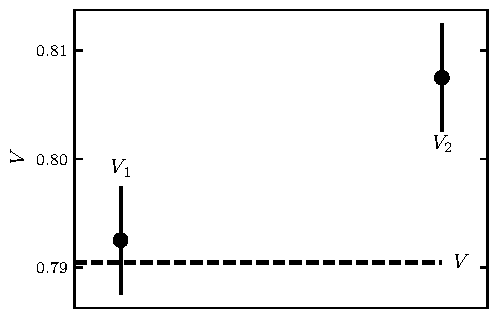
\includegraphics[width=\linewidth]{pdf/original-peelle.pdf}
\caption{Original Peelle problem rewritten in the context of interferometry.  \emph{Bottom:} Two raw visibility amplitudes $\nu_1$ and $\nu_2$ (points with statistic error bars of $\approx 0.6\%$) are calibrated by the transfer function $1/\tau$ (solid line with systematic error zone of 5\%). \emph{Top:} the two calibrated visibility measurements $\data_1$ and $\data_2$ (points with statistic error bars of $\approx 0.6\%$) are strongly correlated. The least-squares estimate for the visibility $\data$ (dashed line, with statistic uncertainty error zone displayed) falls outside of the data range.}
\label{fig:peelle}
\end{figure}

\begin{table}
\caption{Symbols used in this paper. Lower case bold font is used for vectors and upper case bold font for matrices.}
\begin{tabular}{ll}
\hline\hline
Symbol                        & Meaning\\
\hline
$\mean a$                     & true value of $a$\\
$<a>$                         & expectancy of $a$\\
$\tr{\vec A}$                 & transpose of $\vec A$\\
$\vec c = \vec a\hadam\vec b$ & elementwise product of $\vec a$ and $\vec b$\\
$\vec C = \vec a\outer\vec b$ & outer product of $\vec a$ and $\vec b$\\
$\vec c = \vec A\vec b$       & matrix product of $\vec A$ and $\vec b$\\
$\delta$                      & Kronecker delta\\
\hline
$\vdata$                      & data\\ 
$\verror$                     & error ($= \vdata - \vdatamean$)\\
$\dev^2$                      & variance ($= \expect{\error^2}$)\\
$\vcov$                       & covariance matrix ($= \expect{\verror\outer\verror}$)\\
$\corr$                       & correlation coefficient\\
$\vsens$, $\msens$            & sensitivity vector or matrix\\
$\vparam$                     & parameters of the model\\
$\vmod$                       & model values ($= \msens\vparam\approx\vdatamean$)\\
\hline
$a\meas$                      & $a$ of the measurement error\\
$a\norm$                      & $a$ of the normalisation error\\
$\ppp a$                      & $a$ impacted by PPP\\
\hline
\end{tabular}
\end{table}

\section{Single value fit}
\label{sec:single} 

\begin{figure}
\centering
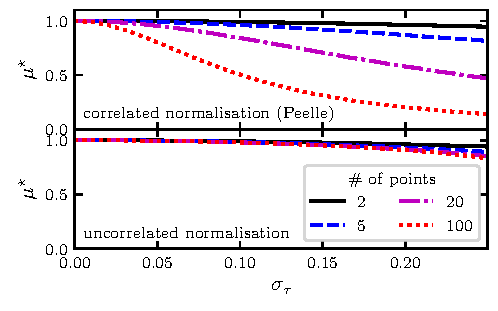
\includegraphics[width=\linewidth]{pdf/uncorrelated-peelle.pdf}
\caption{Fit $\datappp$  to unresolved visibilities ($\data = 1$), as a function of the relative uncertainty on the calibration $\reldev$ and the number of measurements $n$. $2/n\times10^5$ simulations were made and averaged, assuming that $\abserror$ and $\relerror$ follow normal distributions. \textit{Top:} fully correlated normalisation like in original Peelle's puzzle ($\absdev=0.02$ and $\corr = 1$). \textit{Bottom:} normalisation error without correlation ($\absdev=0.02$ and $\corr = 0$).}
\label{fig:uncorr-peelle}
\end{figure}

Let's consider a set of measurements of a single normalised quantity, like the visibility amplitude, given by a column vector $\vdata = \tr{(\data_1, \cdots, \data_n)}$. It is derived from an uncalibrated quantity like the fringe contrast, $\vraw = \tr{(\raw_1, \cdots, \raw_n)}$ and a normalisation factor, like the cotransfer function, $\vcot = \tr{(\cot_1, \cdots, \cot_n)}$ by 
\begin{equation}
    \vdata = \vcot\hadam\vraw,
\end{equation}
where $\hadam$ denotes the Hadamard (elementwise) product of vectors. If $\datamean$, $\cotmean$, and $\rawmean$ the true, but unknown, values of these quantities, the error vector on $\vdata$  
\begin{align}
    \verror    &= \vdata - \datamean, \\
\intertext{can be written as a sum of measurement and normalisation errors if one ignores a second-order term:}
    \verror    &= \vabserror + \datamean \vrelerror.\\
\intertext{These errors are given by}
    \vabserror &= \cotmean (\vraw - \rawmean), \\
    \vrelerror &= \frac1\cotmean (\vcot-\cotmean).
\end{align}

Let's assume $\vabserror$ and $\vrelerror$ are independent error terms of mean 0 and standard deviations are $\absdev$ and $\reldev$, respectively. In addition, I consider correlation of the normalisation errors, with correlation coefficient $\corr$.  In the case of interferometry, it can arise from the uncertainty on the calibrators' geometry.  The covariance matrix is given by
\begin{align}
    \vcov     &= \expect{\verror\outer\verror},\\
\intertext{where $\outer$ denotes the outer product of vectors and $\expect{}$ stands for the expectancy, so that}
    \cov_{ij} &= \left[ \absdev^2 
                  + (1-\corr)\reldev^2\datamean^2
                \right] \delta_{ij} 
            + \corr\reldev^2\datamean^2.
\end{align}

The value $\datamean$ is yet to be determined, so the covariances are often derived using the data in the propagation:
\begin{equation}
    \ppp{\cov_{ij}} = \left[ 
                    \absdev^2 
                  + (1-\corr)\reldev^2 \data_i^2
                \right] \delta_{ij} 
            + \corr\reldev^2\data_i\data_j. \label{eq:cov}
\end{equation}

The least squares estimate for $\datamean$ is given by
\begin{equation}
    \ppp{\mod} =
                  \frac { \tr\vsens{\ppp\vcov}^{-1}\vdata }
                        { \tr\vsens{\ppp\vcov}^{-1}\vsens }
\end{equation}
where $\vsens = \tr{(1, \cdots, 1)}$ is the trivial sensitivity vector.  The covariance matrix is the sum of an invertible diagonal matrix and one of rank one---see \eqref{cov}---, so that the inverse is obtained using the Woodbury matrix identity: 
\begin{align}
    \{ {\ppp\vcov}^{-1} \}_{ij} &= \frac{\delta_{ij}}{\dev_i^2}
         - \frac{\corr\reldev^2\data_i\data_j}
                {\dev_i^2\dev_j^2\Big(1 + 
            \corr\reldev^2\sum\limits_{k} \frac{\data_k^2}{\dev_k^2}\Big)},\\
  \intertext{where}
  \dev_i^2 &= \absdev^2+(1-\corr)\reldev^2\data_i^2.
\end{align}
It allows me to put the least squares estimate in the relatively compact form 
\begin{equation}
  \ppp{\mod} = 
    \frac { 
      \sum\limits_i \frac{\data_i}{\dev_i^2}
    }{ 
      \sum\limits_i 
          \Big( 1   
             + \corr\reldev^2\sum\limits_{j} \frac{(\data_i-\data_j)^2}{\dev_j^2}
           \Big)
          \frac{1}{\dev_i^2} 
   }.\label{eq:mu}
\end{equation}


For small enough errors ($\error_i \ll \datamean$) the second-order Taylor development in $\error_i = \data_i - \datamean$ yields 
\begin{equation}
    \ppp{\mod} \approx  \datamean 
                  +\frac1n {\sum\limits_i \error_i}
                       - \frac {[2 + (n - 2)\corr]\reldev^2\datamean^2
                          }{
                           2n^2 \devmean^2             
                          }
                           \sum\limits_{i\ne j} (\error_i-\error_j)^2
\end{equation}
where
\begin{equation}
    \devmean^2 = \absdev^2+(1-\corr)\reldev^2\datamean^2 
\end{equation}

Since $\expect{\error_i} = 0$ and $\expect{(\error_i-\error_j)^2} = 2\devmean^2$, the expectancy
\begin{equation}
    \expect{\ppp{\mod}} \approx \datamean 
            \left[ 1 -  
             \left(1-\frac1n\right)
             \left(2 + (n-2)\corr\right)
              \reldev^2 \right]
\end{equation}
is biased.  If the data are not correlated ($\corr = 0$), the bias is small
($\reldev^2$ to $2\reldev^2$) but it becomes large for correlated data if the number of points is large ($\sim n\reldev^2$ for fully correlated data) as \citet{DAG94} already noted. Figure~\ref{fig:uncorr-peelle} shows a simulation of the bias as a function of the normalisation uncertainty $\reldev$ for various data sizes ($n = 2$ to 100). 

For spectro-interferometric observations with 4 telescopes, the number of correlated points can be over 1,000, so even with a low correlation coefficient, the impact can be large. For instance, a single GRAVITY observation in high spectral resolution yields $n = 6 \times 210$ visibility amplitudes. With an observed correlation of $\rho \approx 16$\% in the instrumental visibility amplitudes \citep{KAM20} and a typical $\reldev = 1$--2\% normalisation error, the bias on the calibrated visibilities could be 2--8\%.  

\section{Model fitting}
\label{sec:model}

\begin{figure}
\centering
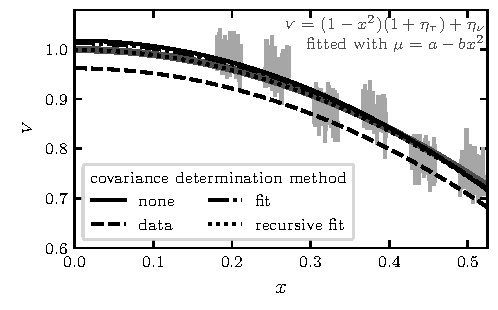
\includegraphics[width=\linewidth]{pdf/fit-example.pdf}
\caption{Example of a fit of correlated data from a four telescope interferometer with medium resolution: 6 groups of 100 data points (light gray points with the measurement error bar) with 2\% uncorrelated measurement errors and 3\% correlated normalisation.  Simulated data follow $\data = 1-x^2$ (thick gray line). Least-squares model fitting $\mod = a-bx^2$ is performed using the four prescriptions for the covariance matrix.}
\label{fig:fitexample}
\end{figure}

\begin{figure*}
\centering
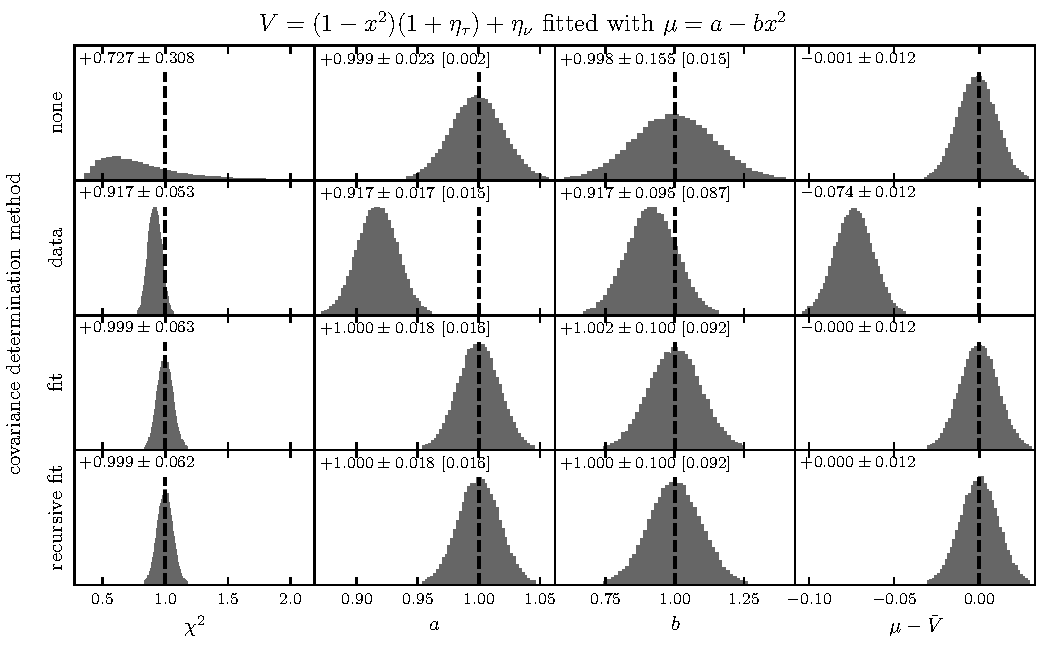
\includegraphics[width=\linewidth]{pdf/fit-quality.pdf}
\caption{Distribution of the fitted parameters and fit properties for the four covariance matrix prescriptions. $5\times10^4$ simulations of 6 groups of 100 correlated data points $\data$ ($\absdev = 2\%$, $\reldev = 3\%$, $\corr = 1$, normal distributions) following $\data = (1-x^2)(1 + \error)+\error$ are performed and fitted with model $\mod = a - bx^2$ using least-squares minimisation. Reported quantities include median and 1-$\sigma$ interval of their distribution and, within brackets, the median uncertainty reported by the least squares fit. \emph{Leftmost column:} distribution of the least squares; \emph{middle left:} constant coefficient $a$; \emph{middle right:} quadadratic coefficient $b$; \emph{rightmost column:} mean difference between model and data. The covariance matrix prescriptions are: \emph{top row:} correlations are ignored; \emph{second row:} a na\"\i{}ve covariance matrix uses the data values; \emph{third row:} covariance matrix uses modelled values from fit without correlations; \emph{bottom row:} covariance matrix and model are recursively computed, with the covariance matrix of the next recursion using the modelled value of the last step.}
\label{fig:fitanalysis}
\end{figure*}

Let's now consider a set of measurements corresponding to the linear model 

\begin{align}
    \vmod  &= \msens\vparam,\\
\intertext{where $\vparam$ are the unknown parameters and $\msens$ is the known sensitivity matrix. Typically, $\sens_{ik}=f_k(u_i, v_i)$ for a linear model and $\sens_{ik} = \partial f/\partial p_k(u_i, v_i)$ for a non-linear model approximated by a linear one close to a solution. $(u, v)$ is the reduced baseline.  The true values $\vdatamean$ are are impacted by errors so that the data are} 
    \vdata &= \vdatamean + \verror\\
\intertext{with the error term $\verror$ again expressed as the sum of a measurement error and a normalisation one:}
    \verror &=  \vabserror + \vrelerror \hadam \vdatamean.
\end{align}
The measurement errors $\vec\abserror$ and normalisation errors $\vec\relerror$ following multivariate distributions of mean zero, with covariance matrices $\vabscov$ and $\vrelcov$ respectively. Given the covariance matrix $\vcov$ of this model, the least squares estimate is
\begin{align}
   \vparam &= (\tr\msens \vcov^{-1} \msens)^{-1} (\tr\msens \vcov^{-1} \vdata)
\end{align}
I investigate four ways to determine the covariance matrix
\begin{enumerate}
    \item Ignoring the correlations in the normalisation using $\vcov_0 = \vabscov + (\vdata\outer\vdata)\hadam(\vrelcov\hadam\vec I)$. Let $\vdataflat = \msens(\tr\msens\vcov_0^{-1}\msens)^{-1}\tr\msens\vcov_0^{-1}\vdata$ the resulting model of the data.\label{item:nocorr} 
    \item Using the na\"\i{}ve estimate $\ppp\vcov = \vabscov + (\vdata\outer\vdata)\hadam\vrelcov$ which is known to lead to Peelle's pertinent puzzle in the trivial case of a constant model.\label{item:ppp}
    \item Using the data model of the fit without the normalisation error: $\vcov_1 = \vabscov + (\vdataflat\outer\vdataflat)\hadam\vrelcov$. This is the generalisation of the two-variables approach by \citet{NEU14}. The resulting least squares model is $\vdatarec{1} = \msens(\tr\msens\vcov_1^{-1}\msens)^{-1}\tr\msens\vcov_1^{-1}\vdata$.\label{item:fit}
    \item Recursively fitting the data by updating the data model in the covariance matrix. I derive $\vdatarec{k} = \msens(\tr\msens\vcov_k^{-1}\msens)^{-1}\tr\msens\vcov_k^{-1}\vdata$ using $\vcov_{k} = \vabscov + (\vdatarec{k-1}\outer\vdatarec{k-1})\hadam\vrelcov$, starting with the estimate $\vdatarec{1}$ ($k = 2$).\label{item:recfit}
\end{enumerate}

In order to compare these covariance matrix prescriptions, I will use the typical example of an under-resolved centrosymmetric source observed at a four-telescope facility in high spectral resolution. In the under-resolved case all models---Gaussian, uniform disc, or limb-darkened disc---are equivalent \citep{LAC03}--- so I will use instead a linear least squares fit $\mod = a - bx^2$ to $\data \approx 1 - x^2$ where $x$ is dimensionless variable proportional to the projected baseline length $\sqrt{u^2+v^2}$. This fit corresponds to the second-order Taylor development of any of the aforementionned models.  Figure~\ref{fig:fitexample} shows the example of such a fit performed for each covariance matrix prescription.  Data has been simulated using $\data = (1-x^2)(1 + \relerror) + \abserror$ where $\relerror$ is a fully correlated normalisation error (3\%) and $\abserror$ are uncorrelated statistical errors (2\%). As expected, the use of data $\vdata$ in the correlation matrix (method \ref{item:ppp}) leads to grossly underestimated data values, in the very same way as in the classical Peelle case described in Sects.~\ref{sec:ppp}~\&~\ref{sec:single}.  Other methods, including ignoring correlations, yield reasonable fits.

Figure~\ref{fig:fitanalysis} sums up the behaviour of the same fit performed a large number of times on different simulated data sets, each following $\data \approx 1-x^2$.  For each correlation matrix prescription, it displays the dispersion of the reduced chi squared, the model parameters $a$ and $b$, and the difference between modelled value and true value. It also reports the uncertainty on model parameters reported by the least squares fit in comparison to the scatter of the distribution of the values. While the model fits ignoring correlations \ref{item:nocorr} does not show any bias, they display a higher dispersion of model parameters and grossly underestimate the uncertainty on model parameters.  The correlation matrix calculated from data \ref{item:ppp} is, as expected, strongly biased. Both methods estimating the correlation  matrix from modelled data, \ref{item:fit} \& \ref{item:recfit}, are equivalent in terms of the absence of bias, dispersion of these quantities, and correct prediction of the uncertainty on model parameters.

Given that fitting recursively the covariance matrix doesn't yield additional benefits, I would suggest to use method \ref{item:fit}.  



\section{Conclusion}

The standard, but incorrect, covariance propagation in any ``normalisation'' setting leads to bias in the model parameters of a least-squares fit taking correlations into account.  Some bias will even occur without correlations, but the effect is strongest when a large set of correlated data is modelled.  This is precisely the case in optical and infrared long-baseline interferometry, where the calibration of spectrally dispersed fringes easily yields $10^2$ to $10^3$ correlated data points.

While solutions exist that are either numerically expensive or require some care to be implemented \citep{BUR11,BEC12,NIS14}, I have shown with a simple example that there is an easy and cheap way to solve the issue. First a uncorrelated fit is performed to estimate the true values corresponding to the data.  Secondly, these estimates are used to determine the covariance matrix by error propagation. At last, this covariance matrix is used to perform a model-fit.




\bibliography{article}

\end{document}
